\documentclass[12pt]{report}
\usepackage[utf8]{inputenc}
\usepackage[T1]{fontenc}
\usepackage[russian]{babel}
%\usepackage[14pt]{extsizes}
\usepackage{multirow}
\usepackage{listings}
\usepackage{graphicx}
\graphicspath{ {./img/} }
\usepackage{amsmath,amsfonts,amssymb,amsthm,mathtools} 
\usepackage[newfloat]{minted}
\usepackage{caption}

\lstset{ %
basicstyle=\small\sffamily, % размер и начертание шрифта для подсветки кода
numbers=left,               % где поставить нумерацию строк (слева\справа)
numberstyle=\tiny,           % размер шрифта для номеров строк
stepnumber=1,                   % размер шага между двумя номерами строк
numbersep=5pt,                % как далеко отстоят номера строк от подсвечиваемого кода
showspaces=false,            % показывать или нет пробелы специальными отступами
showstringspaces=false,      % показывать или нет пробелы в строках
showtabs=false,             % показывать или нет табуляцию в строках
frame=single,              % рисовать рамку вокруг кода
tabsize=2,                 % размер табуляции по умолчанию равен 2 пробелам
captionpos=t,              % позиция заголовка вверху [t] или внизу [b] 
breaklines=true,           % автоматически переносить строки (да\нет)
breakatwhitespace=false, % переносить строки только если есть пробел
escapeinside={\#*}{*)}   % если нужно добавить комментарии в коде
}

% Для измененных титулов глав:
\usepackage{titlesec, blindtext, color} % подключаем нужные пакеты
\definecolor{gray75}{gray}{0.75} % определяем цвет
\newcommand{\hsp}{\hspace{20pt}} % длина линии в 20pt

\titleformat{\chapter}[hang]{\Huge\bfseries}{\thechapter\hsp\textcolor{gray75}{|}\hsp}{0pt}{\Huge\bfseries}

\title{Lab 01 report}
\author{Kirill}

\date{\today}

\begin{document}
\begin{titlepage}
	\centering
	{\scshape\LARGE МГТУ им. Баумана \par}
	\vspace{3cm}
	{\scshape\Large Лабораторная работа №1\par}
	\vspace{0.5cm}	
	{\scshape\Large По курсу: "Анализ алгоритмов"\par}
	\vspace{1.5cm}
	{\huge\bfseries Расстояние Левенштейна\par}
	\vspace{2cm}
	\Large Работу выполнил: Рядинский Кирилл, ИУ7-53Б\par
	\vspace{0.5cm}
	\LargeПреподаватели:  Волкова Л.Л. \par
	
	\vfill
	\large \textit {Москва, 2021} \par
\end{titlepage}


\tableofcontents
\newpage

\chapter*{Введение}
\addcontentsline{toc}{chapter}{Введение}
	
\textbf{Расстояние Левенштейна} - минимальное количество операций вставки одного символа, удаления одного символа и замены одного символа на другой, необходимых для превращения одной строки в другую.

Расстояние Левенштейна применяется в теории информации и компьютерной лингвистике для:

\begin{itemize}
	\item исправления ошибок в слове
	\item сравнения текстовых файлов утилитой diff
	\item в биоинформатике для сравнения генов, хромосом и белков
\end{itemize}

Задачами данной лабораторной являются:
\begin{enumerate}
	\item изучение алгоритмов Левенштейна и Дамерау-Левенштейна нахождения расстояния между строками;
	\item применение метода динамического программирования для матричной реализации указанных алгоритмов; 
	\item получение практических навыков реализации указанных алгоритмов: двух алгоритмов в матричной версии и одного из алгоритмов в рекурсивной версии; 
	\item сравнительный анализ линейной и рекурсивной реализаций выбранного алгоритма определения расстояния между строками по затрачиваемым ресурсам (времени и памяти); 
	\item экспериментальное подтверждение различий во временнóй эффективности рекурсивной и
	      нерекурсивной реализаций выбранного алгоритма определения расстояния между строками при
	      помощи разработанного программного обеспечения на материале замеров процессорного времени
	      выполнения реализации на варьирующихся длинах строк; 
	\item описание и обоснование полученных результатов в отчете о выполненной лабораторной
	      работе, выполненного как расчётно-пояснительная записка к работе. 
\end{enumerate}

\chapter{Аналитическая часть}
Задача по нахождению расстояния Левенштейна заключается в поиске минимального количества операций вставки/удаления/замены для превращения одной строки в другую.

При нахождении расстояния Дамерау — Левенштейна добавляется операция транспозиции (перестановки соседних символов).  
	
\textbf{Действия обозначаются так:} 
\begin{enumerate}
	\item D (англ. delete) — удалить,
	\item I (англ. insert) — вставить,
	\item R (replace) — заменить,
	\item M(match) - совпадение.
\end{enumerate}

Пусть $S_{1}$ и $S_{2}$ — две строки (длиной M и N соответственно) над некоторым алфавитом, тогда расстояние Левенштейна можно подсчитать по следующей рекуррентной формуле:

\begin{displaymath}
	D(i,j) = \left\{ \begin{array}{ll}
	0, & \textrm{$i = 0, j = 0$}\\
	i, & \textrm{$j = 0, i > 0$}\\
	j, & \textrm{$i = 0, j > 0$}\\
	min(\\
	D(i,j-1)+1,\\
	D(i-1, j) +1, &\textrm{$j>0, i>0$}\\
	D(i-1, j-1) + m(S_{1}[i], S_{2}[j])\\
	),
	\end{array} \right.
\end{displaymath}

где $m(a,b)$ равна нулю, если $a=b$ и единице в противном случае; $min\{\,a,b,c\}$ возвращает наименьший из аргументов.

Расстояние Дамерау-Левенштейна вычисляется по следующей рекуррентной формуле:
		    
\[ D(i, j) =  \left\{
	\begin{aligned}
		  & 0, &   & i = 0, j = 0 \\
		  & i, &   & i > 0, j = 0 \\
		  & j, &   & i = 0, j > 0 \\		    	
		&min \left\{
		\begin{aligned}
		&D(i, j - 1) + 1,\\
		&D(i - 1, j) + 1,\\
		&D(i - 1, j - 1) + m(S_{1}[i], S_{2}[i]), \\
		&D(i - 2, j - 2) + m(S_{1}[i], S_{2}[i]),\\
	\end{aligned} \right.
	&& 
	\begin{aligned}
		  & , \text{ если } i, j > 0         \\
		  & \text{ и } S_{1}[i] = S_{2}[j - 1]  \\
		  & \text{ и } S_{1}[i - 1] =  S_{2}[j] \\
	\end{aligned} \\ 
	&min \left\{
	\begin{aligned}
		  & D(i, j - 1) + 1,                         \\
		  & D(i - 1, j) + 1,                         \\
		  & D(i - 1, j - 1) + m(S_{1}[i], S_{2}[i]), \\
	\end{aligned} \right.  &&, \text{иначе}
	\end{aligned} \right.
\]	
	    
\section{Вывод}
В данном разделе были рассмотрены алгоритмы нахождения расстояния Левенштейна и Дамерау-Левенштейна, который является модификаций первого, учитывающего возможность перестановки соседних символов. 
		
\chapter{Конструкторская часть}
\textbf{Требования к вводу}
		
\begin{enumerate}
	\item На вход подаются две строки
	\item uppercase и lowercase буквы считаются разными
\end{enumerate}
		
\textbf{Требования к программе:}

\begin{enumerate}
	\item Две пустые строки - корректный ввод, программа не должна аварийно завершаться
\end{enumerate}

\section{Схемы алгоритмов}
В данной части будут рассмотрены схемы алгоритмов.

\begin{figure}[h]
	\centering
	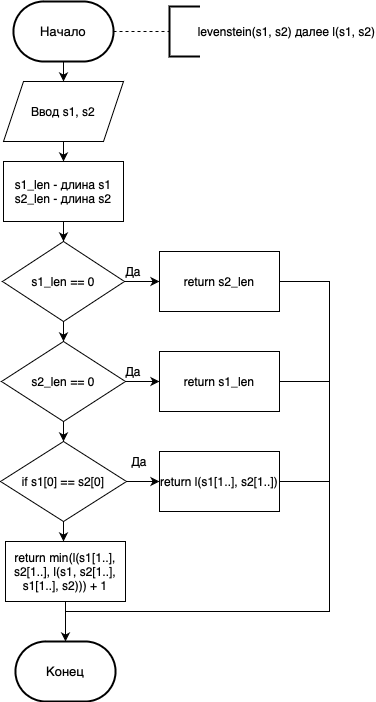
\includegraphics[width=0.5\linewidth]{lev_rec.png}
	\caption{Схема рекурсивного алгоритма нахождения расстояния Левенштейна}
	\label{fig:mpr}
\end{figure}

\begin{figure}[h]
	\centering
	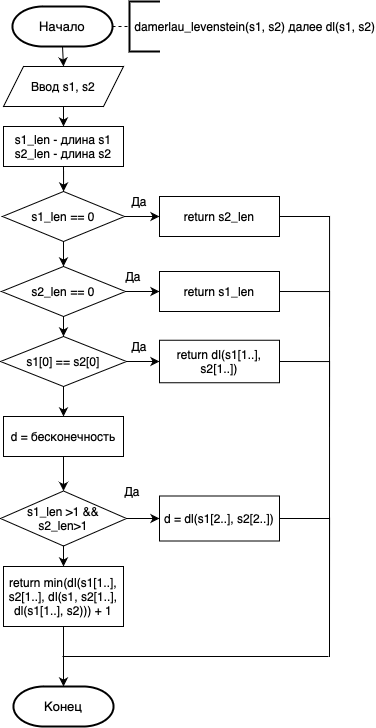
\includegraphics[width=0.5\linewidth]{dam_lev_rec.png}
	\caption{Схема рекурсивного алгоритма нахождения расстояния Дамерау-Левенштейна}
	\label{fig:mpr}
\end{figure}

\begin{figure}[h]
	\centering
	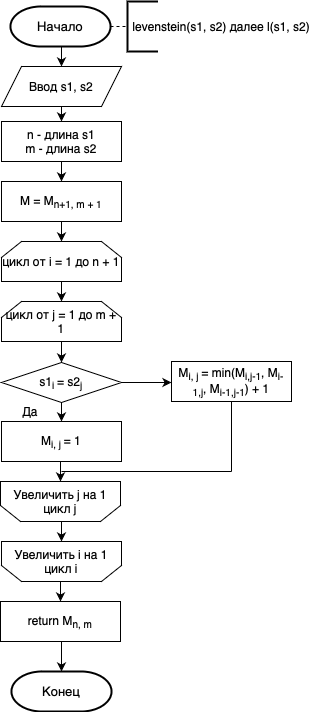
\includegraphics[width=0.6\linewidth]{lev_iter.png}
	\caption{Схема матричного алгоритма нахождения расстояния Левенштейна}
	\label{fig:mpr}
\end{figure}

\begin{figure}[h]
	\centering
	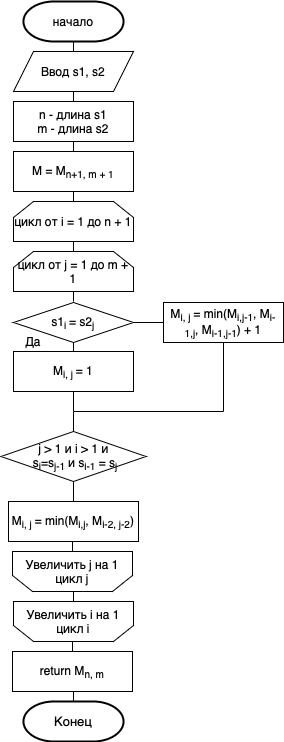
\includegraphics[width=0.5\linewidth]{dam_lev_iter.png}
	\caption{Схема матричного алгоритма нахождения расстояния Дамерау-Левенштейна}
	\label{fig:mpr}
\end{figure}

\chapter{Технологическая часть}
\section{Выбор ЯП}
Для реализации программ я выбрал язык программирования Rust, так как этот язык предоставляет как низкоуровневые интерфейсы, так и высокоуровневые. Также он является таким же быстрым, как и С++, но более безопасен. Среда разработки Visual Studio Code.

\section{Реализация алгоритма}
		
\begin{lstlisting}[label=some-code,caption=Функция нахождения расстояния Левенштейна рекурсивно]
pub fn levenstein_rec(s1: &str, s2: &str) -> usize {
	let s1_len = s1.len();
	let s2_len = s2.len();

	if s1_len == 0 {
		return s2_len;
	}

	if s2_len == 0 {
		return s1_len;
	}   

	if s1.chars().nth(0) == s2.chars().nth(0) {
		return levenstein_rec(&s1[1..], &s2[1..]);
	}

	let a = levenstein_rec(&s1[1..], &s2[1..]);
	let b = levenstein_rec(s1, &s2[1..]);
	let c = levenstein_rec(&s1[1..], &s2);

	return std::cmp::min(a, std::cmp::min(b, c)) + 1;
}
\end{lstlisting}

\newpage

\begin{lstlisting}[label=some-code,caption=Функция нахождения расстояния Дамерау-Левенштейна рекурсивно]
pub fn damerlau_levenstein_rec(s1: &str, s2: &str) -> usize {
	let s1_len = s1.len();
	let s2_len = s2.len();

	if s1_len == 0 {
		return s2_len;
	}

	if s2_len == 0 {
		return s1_len;
	}   

	if s1.chars().nth(0) == s2.chars().nth(0) {
		return damerlau_levenstein_rec(&s1[1..], &s2[1..]);
	}

	let a = damerlau_levenstein_rec(&s1[1..], &s2[1..]);
	let b = damerlau_levenstein_rec(s1, &s2[1..]);
	let c = damerlau_levenstein_rec(&s1[1..], &s2);

	let mut d = usize::MAX;
	if s1_len > 1 && s2_len > 1 {
		d = damerlau_levenstein_rec(&s1[2..], &s2[2..]);
	}

	return std::cmp::min(d, std::cmp::min(a, std::cmp::min(b, c))) + 1;
}

\end{lstlisting}

\newpage

\begin{lstlisting}[label=some-code,caption=Функция нахождения расстояния Левенштейна матрично]
pub fn levenstein_iter(word1: &str, word2: &str) -> usize {
	// getting length of words
	let w1 = word1.chars().collect::<Vec<_>>();
	let w2 = word2.chars().collect::<Vec<_>>();

	let word1_length = w1.len() + 1;
	let word2_length = w2.len() + 1;

	let mut matrix = vec![vec![0; word1_length]; word2_length];

	for i in 1..word1_length {
		matrix[0][i] = i;
	}
	for j in 1..word2_length {
		matrix[j][0] = j;
	}

	for j in 1..word2_length {
		for i in 1..word1_length {
			let x: usize = if w1[i - 1] == w2[j - 1] {
				matrix[j - 1][i - 1]
			} else {
				1 + std::cmp::min(
					std::cmp::min(matrix[j][i - 1], matrix[j - 1][i]),
					matrix[j - 1][i - 1],
				)
			};
			matrix[j][i] = x;
		}
	}
	return matrix[word2_length - 1][word1_length - 1];
}
\end{lstlisting}

\newpage

\begin{lstlisting}[label=some-code,caption=Функция нахождения расстояния Дамерау-Левенштейна матрично]
pub fn damerlau_levenstein_iter(word1: &str, word2: &str) -> usize {
    // getting length of words
    let w1 = word1.chars().collect::<Vec<_>>();
    let w2 = word2.chars().collect::<Vec<_>>();

    let word1_length = w1.len() + 1;
    let word2_length = w2.len() + 1;

    let mut matrix = vec![vec![0; word1_length]; word2_length];

    for i in 1..word1_length {
        matrix[0][i] = i;
    }
    for j in 1..word2_length {
        matrix[j][0] = j;
    }

    for j in 1..word2_length {
        for i in 1..word1_length {
            let x: usize = if w1[i - 1] == w2[j - 1] {
                matrix[j - 1][i - 1]
            } else {
                1 + std::cmp::min(
                    std::cmp::min(matrix[j][i - 1], matrix[j - 1][i]),
                    matrix[j - 1][i - 1],
                )
            };

            matrix[j][i] = x;

            if (j > 1) && (i > 1) && (w1[i - 1] == w2[j - 2]) && (w1[i - 2] == w2[j - 1]) {
                matrix[j][i] = std::cmp::min(x, matrix[j - 2][i - 2] + 1);
            }
        }
    }
    return matrix[word2_length - 1][word1_length - 1];
}
\end{lstlisting}


\begin{table}[h]
	\begin{tabular}{|c|c|c|c|}
	\hline
	\multirow{2}{*}{Строка 1} & \multirow{2}{*}{Строка 2} & \multicolumn{2}{c|}{Ожидаемый результат} \\ \cline{3-4} 
		   &          & Левенштейн & Дамерау-Левенштейн \\ \hline
	Take   & Took     & 3          & 3                   \\ \hline
	Art    & Atr      & 2          & 1                   \\ \hline
	car    & city     & 3          & 3                   \\ \hline
	head   & ehda     & 3          & 2                   \\ \hline
	laptop & notebook & 7          & 7                   \\ \hline
	peek   & peeks    & 1          & 1                   \\ \hline
	rain   & pain     & 1          & 1                   \\ \hline
	\end{tabular}
	\caption{Функциональные тесты}
	\label{tab:func_tests}
\end{table}

В Таблице \ref{tab:func_tests} приведены функциональные тесты для алгоритмов вычисления расстояния Левенштейна и Дамерау-Левенштейна.

\chapter{Исследовательская часть}

\section{Сравнительный анализ на основе замеров времени работы алгоритмов}

Был проведен замер времени работы каждого из алгоритмов.

\begin{table}[h]
	\centering
	\begin{tabular}{ccccc}
	\multicolumn{1}{l}{Длина слов} &
	  \multicolumn{1}{l}{Лев. рек.} &
	  \multicolumn{1}{l}{Лев. итер.} &
	  \multicolumn{1}{l}{Дам. -Лев. рек.} &
	  \multicolumn{1}{l}{Дам. -Лев. итер.} \\ \hline
	\multicolumn{1}{|c|}{1} & \multicolumn{1}{c|}{8,50E-08} & \multicolumn{1}{c|}{2,48E-07} & \multicolumn{1}{c|}{3,20E-10} & \multicolumn{1}{c|}{5,50E-07} \\ \hline
	\multicolumn{1}{|c|}{2} & \multicolumn{1}{c|}{1,08E-07} & \multicolumn{1}{c|}{3,07E-07} & \multicolumn{1}{c|}{4,80E-08} & \multicolumn{1}{c|}{4,93E-07} \\ \hline
	\multicolumn{1}{|c|}{3} & \multicolumn{1}{c|}{3,20E-07} & \multicolumn{1}{c|}{4,26E-07} & \multicolumn{1}{c|}{2,77E-07} & \multicolumn{1}{c|}{4,91E-07} \\ \hline
	\multicolumn{1}{|c|}{4} & \multicolumn{1}{c|}{1,30E-06} & \multicolumn{1}{c|}{4,88E-07} & \multicolumn{1}{c|}{1,50E-06} & \multicolumn{1}{c|}{5,00E-07} \\ \hline
	\multicolumn{1}{|c|}{5} & \multicolumn{1}{c|}{6,90E-06} & \multicolumn{1}{c|}{7,41E-07} & \multicolumn{1}{c|}{8,40E-06} & \multicolumn{1}{c|}{5,08E-07} \\ \hline
	\multicolumn{1}{|c|}{6} & \multicolumn{1}{c|}{3,65E-05} & \multicolumn{1}{c|}{8,12E-07} & \multicolumn{1}{c|}{4,68E-05} & \multicolumn{1}{c|}{5,31E-07} \\ \hline
	\multicolumn{1}{|c|}{7} & \multicolumn{1}{c|}{1,97E-04} & \multicolumn{1}{c|}{9,86E-07} & \multicolumn{1}{c|}{2,64E-04} & \multicolumn{1}{c|}{5,14E-07} \\ \hline
	\multicolumn{1}{|c|}{8} & \multicolumn{1}{c|}{1,00E-03} & \multicolumn{1}{c|}{1,10E-06} & \multicolumn{1}{c|}{1,51E-03} & \multicolumn{1}{c|}{5,20E-07} \\ \hline
	\multicolumn{1}{|c|}{9} & \multicolumn{1}{c|}{5,92E-03} & \multicolumn{1}{c|}{1,22E-06} & \multicolumn{1}{c|}{8,72E-03} & \multicolumn{1}{c|}{5,09E-07} \\ \hline
	\end{tabular}
	\caption{Время работы алгоритмов (в секундах)}
	\label{tab:my-table}
	\end{table}

	\pagebreak
	
	
	\begin{figure}[ht]
		\centering
		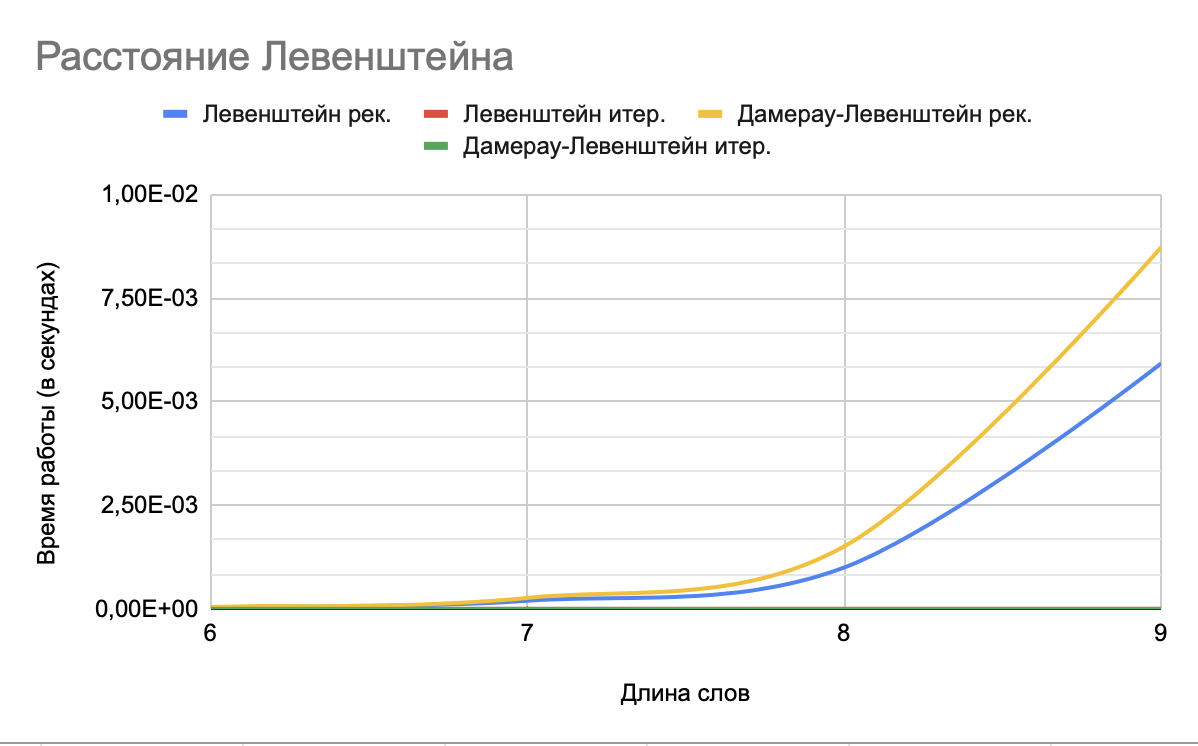
\includegraphics[width=0.75\textwidth]{plot.png}
		\caption{Зависимость времени работы алгоритмов от длины строки.}
		\label{fig:mpr}
	\end{figure}

	Наиболее эффективными по времени при маленькой длине слова являются рекурсивные реализации алгоритмов, но как только увеличивается длина слова, их эффективность резко снижается, что обусловлено большим количеством повторных рассчетов. Время работы алгоритма, использующего матрицу, намного меньше благодаря тому, что в нем требуется только (m + 1)*(n + 1) операций заполнения ячейки матрицы. Также установлено, что алгоритм ДамерауЛевенштейна работает немного дольше алгоритма Левенштейна, т.к. в нем добавлены дополнительные проверки, однако алгоритмы сравнимы по временной эффективности.

	\section{Использование памяти}

	\par
	Алгоритмы Левенштейна и Дамерау-Левенштейна не отличаются по использованию памяти, соответственно достаточно рассмотреть рекурсивный и матричный реализации этих алгоритмов.

	\par
	Максимальная глубина стека вызовов при рекурсивной реализации равна сумме длин входящих строк, соответственно, максимальный расход

	\begin{equation}
		(Size(S_{1}) + Size(S_{2}) \cdot (2 \cdot Size(\text{string}) + Size(\text{int})))
	\end{equation}
	
	\par 
	Где Size - функция, возвращающая размер аргумента; string - строковый тип, int - целочисленный тип.

	\par
	Использование памяти при итеративной реалзиации теоритически равно

	\begin{equation}
		(Size(S_{1} + 1) \cdot Size(S_{2} + 1)) \cdot Size(int) + 2 \cdot Size(string)
	\end{equation}

	\par
	К сожалению, на моей машине не возможны детальные замеры потребления памяти.

	\section{Вывод}

	\par
	Рекурсивный алгоритм Левенштейна работает на порядок дольше итеративных реализаций, время его работы увеличивается в геометрической прогрессии. На словах длиной 9 символов, матричная реализация превосходит рекурсивную в 4800 раз. Рекурсивные алгоритмы Левенштейна и Дамерау - Левенштейна сопостовимы по времени.

	\chapter{Заключение}

	Был изучен метод динамического программирования на материале алгоритмов Левенштейна и Дамерау-Левенштейна.
	Также изучены алгоритмы Левенштейна и Дамерау-Левенштейна нахождения расстояния между строками, получены практические навыки раелизации указанных алгоритмов
	в матричной  и рекурсивных версиях. 

	Экспериментально было подтверждено различие во временной эффективности рекурсивной и нерекурсивной реализаций выбранного алгоритма определения расстояния между строками при помощи разработаного программного обеспечения на материале замеров процессорного времени выполнения реализации на варьирующихся длинах строк. 

	В результате исследований я пришел к выводу, что матричная реализация данных алгоритмов заметно выигрывает по времени при росте длины строк, следовательно более применима в реальных проектах.


\end{document}
